\item \points{15} {\bf Kernelizing the Perceptron}

Let there be a binary classification problem with $y \in \{0, 1\}$.  The
perceptron uses hypotheses of the form $h_\theta(x) = g(\theta^T x)$, where
$g(z) = \text{sign}(z) = 1$ if $z \ge 0$, $0$ otherwise.  In this problem we
will consider a stochastic gradient descent-like implementation of the
perceptron algorithm where each update to the parameters $\theta$ is made using
only one training example.  However, unlike stochastic gradient descent, the
perceptron algorithm will only make one pass through the entire training set.
The update rule for this version of the perceptron algorithm is given by
\begin{equation*}
  \theta^{(i+1)} :=
	  \theta^{(i)} + \alpha (y^{(i+1)} - h_{\theta^{(i)}}(x^{(i+1)})) x^{(i+1)}
\end{equation*}
where $\theta^{(i)}$ is the value of the parameters after the algorithm has
seen the first $i$ training examples. Prior to seeing any training examples,
$\theta^{(0)}$ is initialized to $\vec{0}$.

\begin{enumerate}
  \item \subquestionpoints{9} Let $K$ be a Mercer kernel corresponding to some
very high-dimensional feature
mapping $\phi$. Suppose $\phi$ is so high-dimensional (say,
$\infty$-dimensional) that it's infeasible to ever represent $\phi(x)$
explicitly.  Describe how you would apply the ``kernel trick'' to the
perceptron to make it work in the high-dimensional feature space $\phi$, but
without ever explicitly computing $\phi(x)$.

[\textbf{Note:} You don't have to worry about the intercept term.  If you like,
think of $\phi$ as having the property that $\phi_0(x) = 1$ so that this is
taken care of.] Your description should specify:
\begin{enumerate}[label=\roman*.]
  \item \subquestionpoints{3} How you will (implicitly) represent the
  high-dimensional
    parameter vector $\theta^{(i)}$, including how the initial value
    $\theta^{(0)} = 0$ is represented (note that $\theta^{(i)}$ is
    now a vector whose dimension is the same as the feature vectors
    $\phi(x)$);
  \item \subquestionpoints{3} How you will efficiently make a prediction on a
  new input
    $x^{(i+1)}$.  I.e., how you will compute
    $h_{\theta^{(i)}}(x^{(i+1)}) = g({\theta^{(i)}}^T \phi(x^{(i+1)}))$,
    using your representation of $\theta^{(i)}$; and
  \item \subquestionpoints{3} How you will modify the update rule given above
  to perform an
  update to $\theta$ on a new training example $(x^{(i+1)}, y^{(i+1)})$;
  \emph{i.e.,} using the update rule corresponding to the feature mapping
  $\phi$:
  \begin{equation*}
  \theta^{(i+1)} :=
	  \theta^{(i)} + \alpha (y^{(i+1)} - h_{\theta^{(i)}}(x^{(i+1)})) x^{(i+1)}
  \end{equation*}
\end{enumerate}

\ifnum\solutions=1 {
  \begin{answer}
    \begin{enumerate}
        \item The recursive form of $\theta^{(i+1)}$ suggested that each $\theta^{(i+1)}$ can be represented as a linear combination of $\phi(x^{(1)}), \ldots, \phi(x^{(i)})$. For convenience, we can represent $\theta^{(i)}$ as a $m$-dimensional vector $\gamma^{(i)}$ ($m$ is the number of traning examples), and $\gamma^{(i)}_j$ will be the coefficient of $\phi(x^{(j)})$. $\theta^{(0)}$ can be represented as $\lambda^{(0)} = \vec{0}$.
            In practice, the vector can be implemented as a variable-length list. Then $\theta^{(0)}$ will just be an empty list.
        \item To compute $(\theta^{(i)})^T\phi(x^{(i+1)})$, You first compute $K_j = K(x^{(j)}, x^{(i+1)})$ for each $j$, then compute $g((\lambda^{(i)})^T K)$. Note a list implementation can be more efficient.
        \item Consider $\lambda^{(i+1)}$. First set $\lambda^{(i+1)} = \lambda^{(i)}$, and then set $\lambda^{(i+1)}_{i+1} = \alpha(y^{(i+1)} - g((\theta^{(i)})^Tx^{(i+1)})$. 

    \end{enumerate}
\end{answer}

} \fi


\ifnum\solutions=1 {
  \begin{answer}
    \begin{enumerate}
        \item The recursive form of $\theta^{(i+1)}$ suggested that each $\theta^{(i+1)}$ can be represented as a linear combination of $\phi(x^{(1)}), \ldots, \phi(x^{(i)})$. For convenience, we can represent $\theta^{(i)}$ as a $m$-dimensional vector $\gamma^{(i)}$ ($m$ is the number of traning examples), and $\gamma^{(i)}_j$ will be the coefficient of $\phi(x^{(j)})$. $\theta^{(0)}$ can be represented as $\lambda^{(0)} = \vec{0}$.
            In practice, the vector can be implemented as a variable-length list. Then $\theta^{(0)}$ will just be an empty list.
        \item To compute $(\theta^{(i)})^T\phi(x^{(i+1)})$, You first compute $K_j = K(x^{(j)}, x^{(i+1)})$ for each $j$, then compute $g((\lambda^{(i)})^T K)$. Note a list implementation can be more efficient.
        \item Consider $\lambda^{(i+1)}$. First set $\lambda^{(i+1)} = \lambda^{(i)}$, and then set $\lambda^{(i+1)}_{i+1} = \alpha(y^{(i+1)} - g((\theta^{(i)})^Tx^{(i+1)})$. 

    \end{enumerate}
\end{answer}

} \fi

  \clearpage
\item \subquestionpoints{10} \textbf{Coding problem.}
We will now consider the following dataset (the
formatting matches that of Datasets 1-4, except $x^{(i)}$ is 1-dimensional):
\begin{center}
	\url{data/ds5_{train,valid,test}.csv}	
\end{center}
In \texttt{src/p05b\_lwr.py}, implement locally weighted linear regression
using the normal equations you derived in Part (a) and using
%
\begin{equation*}
	w^{(i)} = \exp\left(-\frac{\|x^{(i)} - x\|_2^2}{2\tau^2}\right).
\end{equation*}
%
Train your model on the \texttt{train} split using $\tau = 0.5$, then run your
model on the \texttt{valid} split and report the mean squared error (MSE).
Finally plot your model's predictions on the validation set (plot the
training set with blue `x' markers and the validation set with a red `o'
markers). Does the model seem to be under- or overfitting?

\ifnum\solutions=1 {
  \begin{answer}
\end{answer}

} \fi


\ifnum\solutions=1 {
  \begin{answer}
\end{answer}

} \fi


  \item \subquestionpoints{2} 
One of the choices in Q4b completely fails, one works a bit, and one works well in classifying the points.
Discuss the performance of different choices and why do they fail or perform well?



\ifnum\solutions=1 {
  \begin{answer}
    \begin{figure}[htbp]
        \begin{subfigure}[b]{0.5\linewidth}
            \centering
            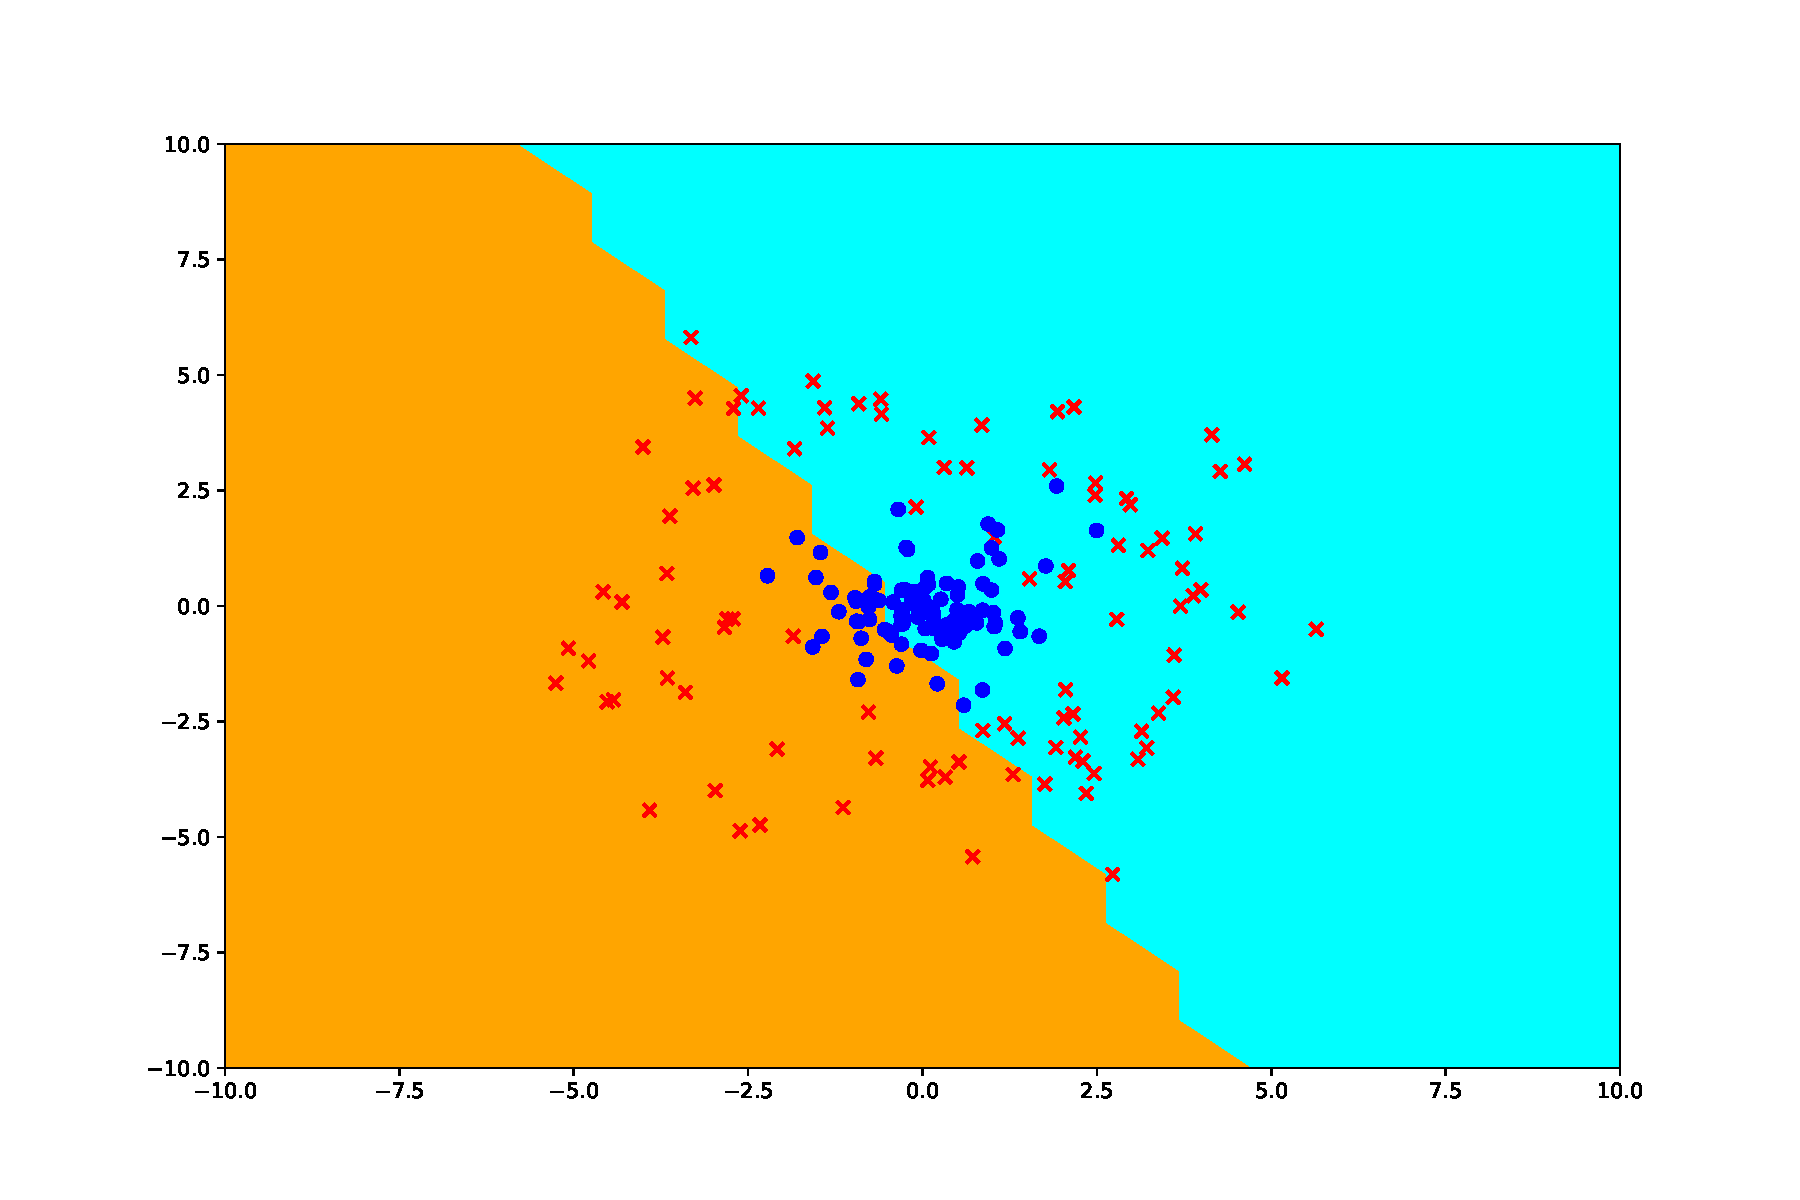
\includegraphics[width=\linewidth]{pics/p05_dot_output.pdf}
            \caption{Dot}
        \end{subfigure}
        \begin{subfigure}[b]{0.5\linewidth}
            \centering
            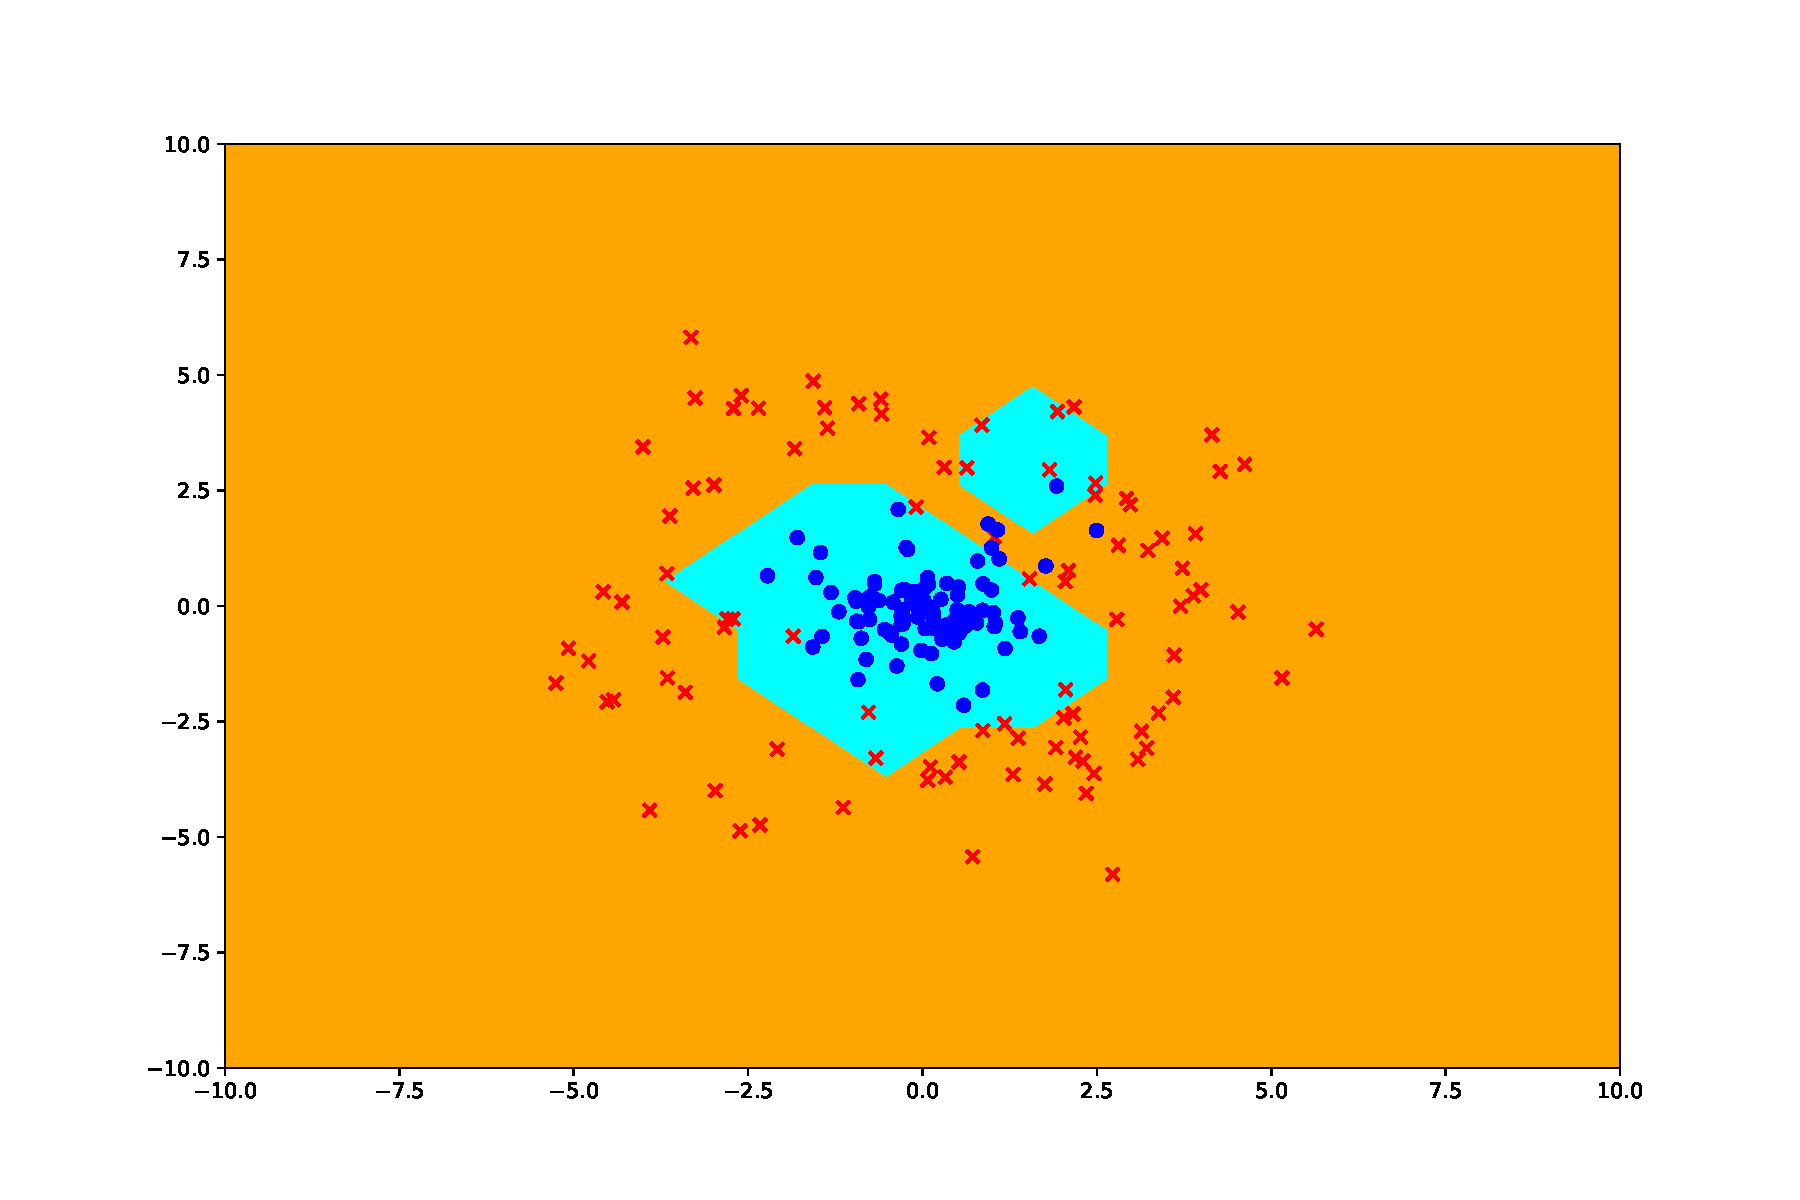
\includegraphics[width=\linewidth]{pics/p05_rbf_output.pdf}
            \caption{RBF}
        \end{subfigure}
    \end{figure}

    The fist performs poorly because using dot product it is equivalent to use $\phi(x^{(i)}) = x^{(i)}$, but the data is not linearly seperable.
\end{answer}

} \fi

\end{enumerate}
